\section{Colhendo dados reais - Arduino}\label{arduino}

Para coletar os dados expostos será necessário o uso de um microcontrolador que tenha um conversor analógico-digital para mensurar os níveis de intensidade da luz projetados pelo laser após a fenda. Para tal atividade, será utilizado um kit UNO Arduíno e os dados serão transmitidos através de uma comunicação serial RS232.

%\section{Programando o Arduino}\label{arduino}

\subsection{Levantando o programa}\label{program_arduino}

Inicialmente, é importante frisar que o kit do Arduíno nada mais é que uma camada de abstração criada acima do microcontrolador AVR. Desta forma, podemos programar nos kits do Arduíno de duas formas sob o sistema Linux:

\subsubsection{Shield Comum}\label{noob}

A forma mais simples de utilizar um kit do Arduíno é utilizando a própria IDE oferecida para o kit. A sua instalação é bem simples e fácil de ser feita. Basta entrar com o seguinte comando no terminal:


\begin{lstlisting}[style=Bash,numbers=none]
user@DESKTOP: sudo apt-get install arduino
\end{lstlisting}

Desta forma, podemos acessar a IDE do Arduíno, que pode ser observada na figura \ref{arduino_ide} e escrever o programa tranquilamente, utilizando apenas as funções $loop$ e $setup$.

\end{multicols}
\begin{figure}[H]
\begin{center}
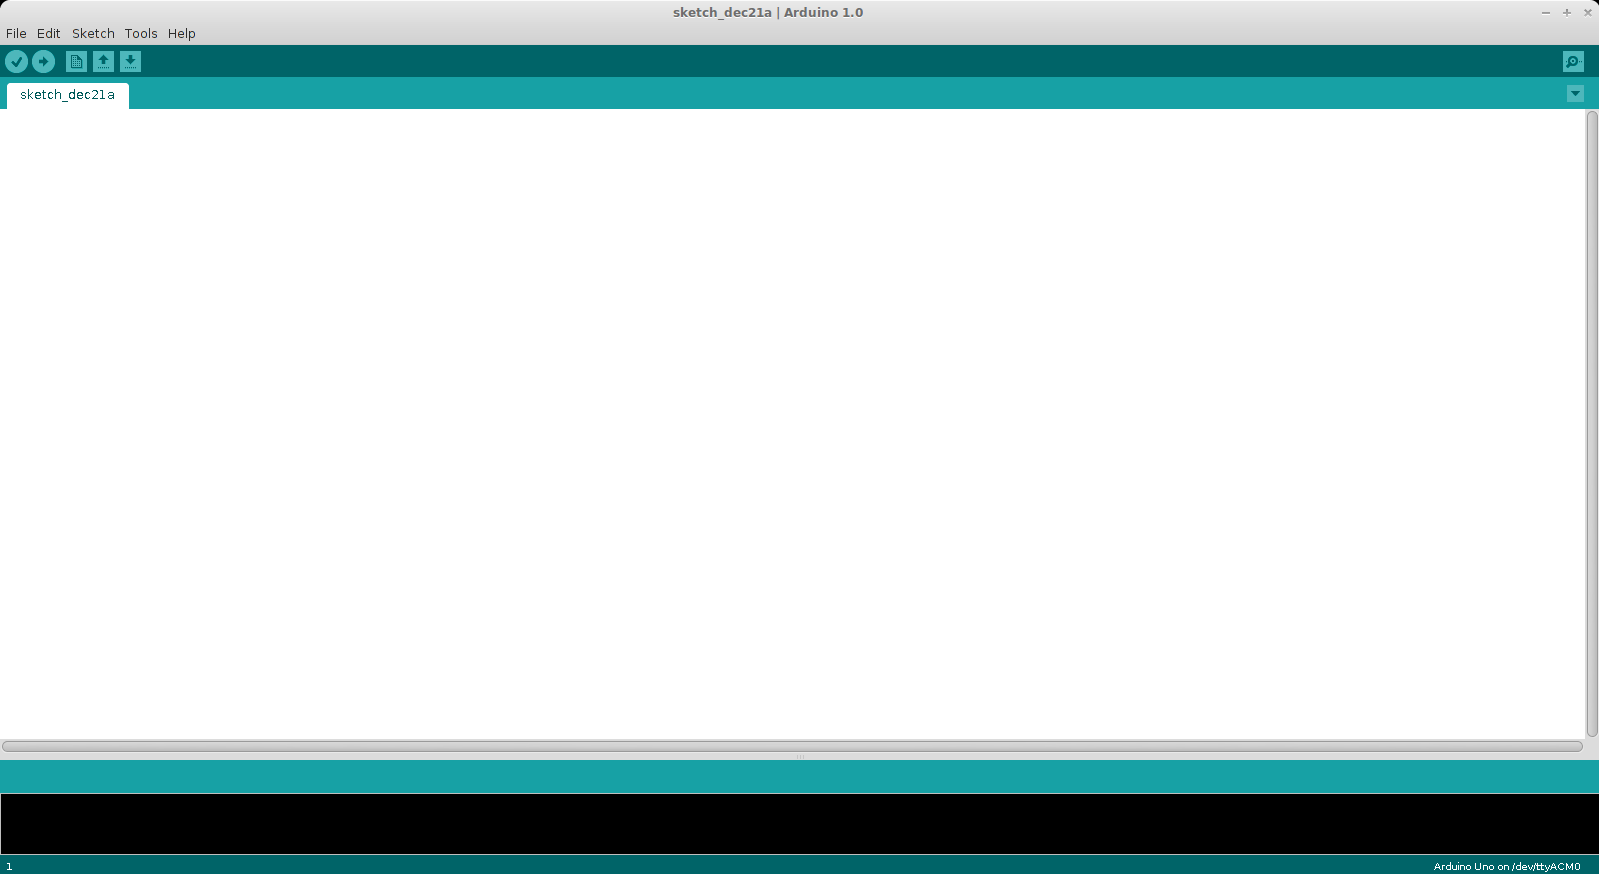
\includegraphics[scale=0.25,angle=0,keepaspectratio=true]{./fts/arduino_ide.png}
\end{center}
\caption{IDE do Arduino}
\label{arduino_ide}
\end{figure}
\begin{multicols}{2}    % 2 columns

\subsubsection{Utilizando o Eclipse para o Arduino}\label{eclipse}

Porém há alguns grandes inconvenientes ao utilizar a IDE do Arduino.

\begin{itemize}
	\item Todas as bibliotecas serão compiladas sempre
	\item O editor de texto deixa muito a desejar
	\item Não há uma função de auto-completar para facilitar o uso das funções já criadas
\end{itemize}

Desta forma, uma opção interessante é utilizar o Eclipse para programar o Arduíno. Isso requer alguns conceitos mais avançados de programação que não serão descritos neste relatório, que são eles:

\begin{itemize}
	\item Instalação do \textit{avr-gcc} e \textit{avrdude}
	\item Criação de uma biblioteca estática com os arquivos em $/usr/shared/arduino$.
	\item Inclusão do diretório $/usr/shared/arduino$ nas dependências da compilação.
	\item Configuração da compilação com as flags $-Os$,$-O3$ e $-g$.
	\item Instalação do plugin de AVR e do AVRDude no Eclipse.
\end{itemize}

Um passo a passo de como proceder com a configuração do Eclipse para uso do Arduíno pode ser observado em \cite{eclipse}.

Outro fator interessante de se usar o Eclipse é a necessidade de fazer uma função $main$, já que esta é descartada pela IDE do Arduíno. Abaixo segue um exemplo de como a função $main$ poderia ser escrita para ter um funcionamento semelhante ao da IDE do Arduíno, facilitando assim a compatibilidade entre os códigos.

%\end{multicols}
\begin{lstlisting}[basicstyle=\ttfamily,numbers=none,caption={[Exemplo da função main()]Código de exemplo da função main()}]

#include <Arduino.h>

int main(void)
{

	init();
	setup();

	while(true) 
		loop();

	return 0;
}
\end{lstlisting}
%\begin{multicols}{2}    % 2 columns

Observe que este código mantem toda a estrutura básica do Arduíno, assim como a inclusão do header $Arduino.h$, necessário para a inclusão das rotinas básicas do Arduíno, assim como sua configuração.

\subsection{Criação do Código}\label{making_arduino}

Com o ambiente de trabalho já configurado, o próximo passo é levantar o programa que funcione de acordo com o diagrama, apresentado na figura \ref{flux_micro}.

\begin{figure}[H]
\begin{center}
\begin{tikzpicture}[node distance = 2cm]
	\tiny\ttfamily
	%-- Estados
	\node [cloud] (init) at(0,0) {Inicio};
	\node [estado] (E1) at(2,0) {Inicializa\\ UART e ADC};
	\node [estado] (E2) at(4,0) {Captura ADC};
	\node [estado] (E3) at(4,-2) {Escreve ADC na UART};
	%-- Setas
	\path (init) edge [line] (E1);
	\path (E1) edge [line] (E2);
	\path (E2) edge [bend right,->] (E3);
	\path (E3) edge [bend right,->] (E2);
\end{tikzpicture}
%\\\hypertarget{diagrama}{Fluxograma do microcontrolador}
\end{center}
\caption{Fluxograma do microcontrolador}
\label{flux_micro}
\end{figure}

Como descrito no diagrama, é necessário inicializar tanto a UART (Comunicação Serial) quanto o ADC (Conversor Analógico-Digital) antes de prender o microcontrolador no laço infinito de captura e exportação dos valores do ADC. Seguindo o contexto de manter a máxima semelhança com o modelo proposto de programação no Arduino, inicializaremos a UART e o ADC na função $setup$ da seguinte forma:

\begin{lstlisting}[basicstyle=\ttfamily,numbers=none,caption={[setup()]Código da função setup()}]

void setup()
{
	Serial.begin(9600);
	analogReference(EXTERNAL);
}

\end{lstlisting}

Observe que a UART é inicializada com rate de 9600, enquanto o conversor é configurado para usar a referencia de tensão externa. A velocidade de 9600 é uma faixa de velocidade bem comum em comunicações seriais. Já a referencia externa é necessária devido ao circuito que foi proposto na sessão \ref{cirt_final_sec}, onde a figura \ref{final} apresenta uma tensão de referencia.

Com o chip já configurado, o próximo passo é configurar a função $loop$ para que o processo de captura do valor do ADC e impressão deste valor seja mantido enquanto o chip estiver alimentado.



\begin{lstlisting}[basicstyle=\ttfamily,numbers=none,caption={[loop()]Código da função loop()}]

void loop()
{
static int i=0;
char buf[20];

	sprintf(buf,"%d %d\n",
		i++,analogRead(0));
	Serial.print(buf);
}
\end{lstlisting}

Desta forma, os valores serão impressos na porta serial com a formatação \textit{"x y"}, estando assim prontos para serem plotados no GNUPLOT. No apêndice \ref{src} pode-se observar na integra este código no Listing
\ref{main_c}, onde haverá a inclusão de alguns headers e alguns tempos no decorrer do programa para garantir uma maior estabilidade do código.



\section{Coletando os dados no computador - Python}\label{python}

Com o processo realizado na sessão \ref{arduino}, qualquer equipamento capacitado para a leitura de comunicação serial poderá realizar a leitura dos dados. Trabalhar com os dados no computador é incrivelmente mais fácil que em um microcontrolador. A taxa de processamento e a memoria disponível são extremamente maiores, sem dizer que as camadas de abstração existentes facilitam - e muito - o nosso trabalho. Isso poderá ser observado através do método que será utilizado para esta etapa. O objetivo é criar um programa em Python que faça a leitura dos dados na porta serial e exporte-os para o GNUPLOT, plotando o gráfico.

\subsection{Python - o inicio}\label{python1}

Python é uma linguagem interpretada orientada à objetos que, normalmente, já vem pré-instalada em grande parte das distribuições Linux. É uma linguagem consideravelmente fácil de ser aprendida e que poder ser incrivelmente útil e pratica. Para este nosso experimento, utilizaremos uma biblioteca do Python chamada \textit{\cite{pyserial}pyserial}, uma biblioteca voltada para a recepção e envio de dados através de comunicações seriais.

Inicialmente, assim como em quase toda lingaugem de programação, iniciamos incluindo as bibliotecas que serão necessárias no decorrer do programa:


\begin{lstlisting}[basicstyle=\ttfamily,language=Python,numbers=none,caption={[Bibliotecas do Python] Inclusão das bibliotecas do Python}]

#!/usr/bin/python
import serial
import os
import subprocess
import sys

\end{lstlisting}

o trecho \lstinline [basicstyle=\ttfamily,language=Python]{#!/usr/bin/python} é muito comum é scripts em ambiente Linux. Quando colocados na primeira linha, este trecho possibilita que ao darmos direitos de execução ao script ( torna-lo executável), ele irá procurar pelo binario, em \textit{/usr/bin/python} no caso, para ser executado. Essa linha nos permite não ter que dar o trabalho de invocar o programa python, já que o script se encarregaria disto.

Em seguida, devemos tentar abrir a porta na qual desejamos escutar. Para uma maior portabilidade do código, o programa foi montado de forma que o parâmetro enviado junto com a inicialização do script seria o endereço desejado, como pode-se ver logo abaixo:

\begin{lstlisting}[basicstyle=\ttfamily,language=Python,numbers=none,caption={[Acessando a porta serial]Acessando a porta serial}]

try:
	ser = serial.Serial(sys.argv[1],9600)
	ser.open()
except IndexError:
	print "Passe uma porta existente 
		com o parametro!"
	sys.exit(0)

f=file('./saida.txt','w')

\end{lstlisting}
Com um conhecimento básico em orientação à objetos, conseguimos ver o quanto Python é intuitivo. Observe que o programa esta atrelado a uma velocidade de comunicação de 9600, assim como o código do arduino foi feito, na sessão \ref{making_arduino}.

\subsection{Lendo os dados}\label{reading}


Caso o programa consiga abrir a porta, devemos então começar a lê-la. Porém em momento algum foi dito quantos dados seriam lidos pela porta serial. Uma forma banal de contornar isto seria arbitrar um valor qualquer de leituras, mas há uma forma mais refinada de contornar este problema.

Assim como em C, podemos trabalhar com interrupções do sistemas em Python. O que faremos então é manter o código preso em um laço infinito lendo as informações e gravando-as em um arquivo, enquanto não ocorrer uma interrupção do teclado (\textit{KeyboardInterrupt}).

\begin{lstlisting}[basicstyle=\ttfamily,language=Python,numbers=none,caption={[Lendo dados]Lendo dados ininterruptamente}]

print "Aperte Ctrl+C para terminar a leitura\n\n"
while True:
	try:
		msg = ser.readline()
		print msg 
	except KeyboardInterrupt:
		print "\rFim da leitura!"
		break	
	finally:
		f.write(msg)
		ser.close()

\end{lstlisting}

\subsection{Plotando os dados}\label{plotting}


Observe que após este passo teremos um arquivo com todos os dados coletados e já com a formatação desejada pelo GNUPLOT, tudo o que temos que fazer é invocar o GNUPLOT e plotar o arquivo, algo que podemos fazer facilmente dentro do próprio Python:

\begin{lstlisting}[basicstyle=\ttfamily,language=Python,numbers=none,caption={[Plotando os dados]Plotando os dados através do Python}]

proc = subprocess.Popen(['gnuplot','-p'], 
                        shell=True,
                        stdin=subprocess.PIPE,
                        )
                        
proc.stdin.write("plot 'saida.txt' with lines\n")
proc.stdin.write("pause mouse\n")
proc.stdin.write("quit\n")

\end{lstlisting}

Com isso, teremos ao final do script um gráfico plotado na tela com os valores coletados pela porta serial. No apêndice \ref{src} pode-se observar na integra este código no Listing
\ref{main_py}, onde haverá a inclusão de alguns  comentários no código e interação com o usuário.
